\title{\dlo{Semi-automatic d}\wen{D}ip-separated structural filtering using seislet transform and adaptive empirical mode decomposition based dip filter}

\renewcommand{\thefootnote}{\fnsymbol{footnote}}
\author{Yangkang Chen}

\address{
\footnotemark[1]Bureau of Economic Geology \\
John A. and Katherine G. Jackson School of Geosciences \\
The University of Texas at Austin \\
University Station, Box X \\
Austin, TX 78713-8924 \\
ykchen@utexas.edu
}

\lefthead{Chen}
\righthead{Dip-separated structural filtering}
\maketitle

% for multiple-revision
\DeclareRobustCommand{\dlo}[1]{\ifthenelse{\boolean{@revd}}{}{}}
\DeclareRobustCommand{\wen}[1]{%
  \ifthenelse{\boolean{@revd}}{\textcolor{black}{#1}}{#1}}
  
\begin{abstract}
The seislet transform has been demonstrated to have a better compression performance for seismic data compared with other well-known sparsity promoting transforms, thus it can be used to remove random noise by simply applying a thresholding operator in the seislet domain. Since the seislet transform compresses the seismic data along the local structures, the seislet thresholding can be viewed as \dlo{the simplest}\wen{a simple} structural filtering approach. Because of the dependence on a precise local slope estimation, the seislet transform usually suffers from low compression ratio and high reconstruction error for seismic profiles that have dip conflicts. In order to remove the limitation of seislet thresholding in dealing with conflicting-dip data, I propose a \dlo{semi-automatic} dip-separated filtering strategy. In this method, I first use an adaptive empirical mode decomposition based dip filter to separate the seismic data into several dip bands (5 or 6)\dlo{, and then I manually recombine the decomposed dip components into a small number (2 or 3) of dip components in order to reduce computational cost}. Next, I apply seislet thresholding to each separated dip component \dlo{(after dip recombination)} to remove random noise. Then I combine all the denoised components to form the final denoised data. \dlo{There are two combination steps in the multi-step process: the dip combination after empirical mode decomposition based dip filtering and the combination of denoised components to form the output data.} Compared with other dip filters, the empirical mode decomposition based dip filter is data-adaptive. One only need to specify the number of dip components to be separated. \dlo{There is only one manual step in the proposed denoising framework; the manual combination of dip components after the initial dip filtering. Thus the semi-automatic multi-step approach is easy to be implemented.} Both complicated synthetic and field data examples show superior performance of my proposed approach than the traditional alternatives. The dip-separated structural filtering is not limited to seislet thresholding, and can also be extended to all those methods that require slope information.
\end{abstract}

\section{Keywords}
\dlo{Semi-automatic d}\wen{D}ip-separated structural filtering, seislet thresholding, empirical mode decomposition, dip filter


\section{INTRODUCTION}
Random noise attenuation is \dlo{one of the principal problems}\wen{an important task} in seismic data processing \wen{\cite[]{fxydecon,ramesh2006,guochang20112,guochang2012,sanyi2012,wencheng2015asa,shuwei20152,weilin2015,qushan2015}}. Among different random noise attenuation approaches, the transform domain thresholding \wen{approach} is \wen{one of the most} widely-known \wen{approaches} \cite[]{yangkang2016dsd}. The principle of this type of approach is simple: seismic reflection has coherent structure and can be sparsely represented while random noise are spreading through the whole transform domain, thus random noise can be removed by applying a simple thresholding operator in the transformed domain. One of the most well-known \dlo{and robust} transforms might be \wen{the} Fourier transform, or $f$-$k$ transform. linear events are transformed into narrow strings in the $f$-$k$ domain. The basic assumption of using $f$-$k$ transform based thresholding is that the \dlo{seismic events should be linear}\wen{data is built of monochromatic plane waves}. To consolidate the assumption, windowed $f$-$k$ transform is usually used to ensure the linear property of local seismic events. Another emerging sparsity-promoting transform is Radon transform. According \wen{to} the shape of the integral operator in the Radon transform, Radon transform can be divided into different types. Among the most popular types are linear Radon transform (also known as slant stack), parabolic Radon transform, hyperbolic Radon transform, and polynomial Radon transform \wen{\cite[]{yaru2014,yaru2016demul}}. As the standard Radon transform operator is not unitary, least-squares and high-resolution version\wen{s} of Radon transform are often used to ensure a practical application of \wen{the} Radon transform. The basic assumption \dlo{beyond}\wen{behind the} Radon transform based thresholding is that the shape of seismic events follows the shape of the integral operator that is used in the Radon transform. \dlo{Curvelet}\wen{The curvelet} transform is becoming more and more popular in \dlo{exploration geophysics field}\wen{the field of exploration geophysics} because of its multi-dimensional and multi-scale \dlo{structures}\wen{properties} \cite[]{hennenfent2006,neelamani2008,neelamani2010,liuwei20162}. \wen{The curvelet transform can give a very sparse representation of a seismic wavefield which has advantages for interpolation and denoising of these data \cite[]{hermann2007}. Therefore it has become more and more popular in exploration geophysics in recent years.} Because \dlo{of the sophisticated construction of}\wen{the} curvelet transform takes both the direction and scale into account, \dlo{curvelet transform}\wen{it} can \dlo{be more adaptive}\wen{get sparser representation for complex data} than many other alternatives. \dlo{The assumption behind the curvelet transform is that the image should have local-symmetric structure.} \wen{The curvelet transform does not have any a prior knowledge of the seismic data, which is designed for a general image processing task. Recently popular shearlet transform is also a natural extension of wavelet transform to accommodate the fact that multivariate functions are typically governed by anisotropic features such as edges in images.} All of the aforementioned sparsity-promoting transforms are \dlo{parameters dependent}\wen{parameter-dependent}, rather than data dependent. \wen{For example, the good compression performance using curvelet transform depends on the input parameters, such as the scales and the directions, while the seislet transform only depends on the local slope that is estimated directly from the data.} 

\dlo{Different from images from the digital signal processing field, seismic images have well-constructed geological structures (e.g. coherent along the spatial dimension), and thus are suitable for structural filtering in order to enhance useful signals and removing noise . However, structural filtering usually requires a precise local slope estimation, which can be demanding in complex seismic profiles because of the difficulty in calculating conflicting dips.} 
 
\cite{seislet} propose a wavelet-like transform that is tailed especially \dlo{for}\wen{to} seismic data, called seislet transform. The seislet transform follows the lifting scheme \cite[]{sweldens1995} in constructing the second generation wavelet transform. The only difference between \wen{the} seislet transform and the general second-generation wavelet transform is that the prediction operator in the seislet transform framework is \wen{defined as} the prediction between different traces according to local slope. The key component of \wen{the} seislet transform is the estimation of local slope of seismic data using plane-wave destruction algorithm. The seislet transform is a\dlo{n} \dlo{outbreak}\wen{breakthrough} in the development of fixed basis sparsity promoting transforms because it can be data adaptive as long as the slope estimation is up to a certain degree of accuracy. \wen{The s}\dlo{S}eislet transform has been successfully used in random noise attenuation, seismic data interpolation, stacking without estimating \dlo{RMS}\wen{the normal-moveout} velocity \cite[]{seislet}, and separation of simultaneous-source seismic data. \wen{As the seislet transform compresses the seismic data along local structures, thus seislet thresholding \cite[]{seislet} can be considered as the simplest structural filtering approach.} \wen{Different from images from \wen{the} digital signal processing field, \dlo{the }seismic images have well-constructed geological structures (e.g. coherent along the spatial dimension), and thus are suitable for structural filtering in order to enhance useful signals and removing noise \cite[]{hale2011,shuwei2015,wencheng2015stack,zhiguang2016}. However, structural filtering usually requires a precise local slope estimation, which can be demanding in complex seismic profiles because of the difficulty in calculating conflicting dips. }

Because of the close \dlo{dependency}\wen{dependence} on slope estimation, \wen{the} seislet transform can be limited \dlo{sometimes} to \dlo{real}\wen{practical} application\wen{s} for some specific datasets when slope estimation is not acceptable, such as dip-conflicting profiles and highly noisy profiles. In order to solve this problem, several alternatives to \wen{the} plane-wave destruction based seislet transform have been proposed. \cite{liuyang2010} proposed the offset continuation based seislet transform. In \wen{the} offset continuation based seislet transform, \wen{the} offset continuation operator is used as \wen{a} replacement of \dlo{PWD}
\wen{plane-wave destruction} operator for the prediction between different traces. The offset continuation operator can only be used to predict traces along the offset direction because of the sole continuation direction \wen{but cannot be used to predict traces along the midpoint direction}, thus it can\dlo{ }not be used in image domain (common offset gathers). \cite{liuyang2013} introduced the velocity dependent seislet transform. \wen{The} \dlo{V}\wen{v}elocity dependent seislet transform use\wen{s} normal-moveout based velocity analysis to obtain velocity spectra and transform\wen{s} the normal-moveout velocity to local slope \dlo{that}\wen{which} is required by the plane-wave destruction based seislet transform. However, the velocity dependent seislet transform can only be applied in common midpoint gathers \wen{since one cannot apply NMO-based velocity analysis in common offset gathers}. The problem of estimating correct local slope in common offset gathers, or stacked image, is still an unsolved problem. 

Empirical mode decomposition (EMD) based dip filter was first proposed by \cite{yangkang2014}. The EMD based dip filter is a data-driven adaptive dip filter. EMD based dip filter utilizes EMD in each frequency slices to separate different spatial oscillating (wavenumber) components that corresponds to different dip components. Because of the adaptive property, the only parameter\dlo{s} \dlo{I}\wen{one} need to define is the number of dip components. \cite{yangkang2014} utilized \dlo{EMDBDF}\wen{EMD based dip filter} to improve the \dlo{predictive}\wen{denoising} performance of $f$-$x$ predictive filtering. $f$-$x$ EMD filtering can also be understood \dlo{using}\wen{as} \wen{EMD based dip filter} considering that random noise\dlo{ and}\wen{,} steeply dipping coherent events and ground rolls can be removed by applying a high-cut \dlo{EMDBDF}\wen{EMD based dip filter}, as mentioned in \cite[]{yangkang2014}. 

In this paper, I propose \dlo{a semi-automatic}\wen{an effective} way to solve the conflicting-dip problem of many structural filtering  by separating different dips of the seismic image first, and then applying the structural filtering to each dip-separated gather secondly. \dlo{We}\wen{I} take the seislet thresholding as \dlo{the simplest}\wen{an} example to show the philosophy of the proposed methodology. When dip conflicts exist, the seislet transform can\dlo{ }not get a good compression performance. For this case, I first apply an EMD based dip filter to separate the seismic data into different \dlo{initial} dip components\dlo{, then I manually combine the initially separated dip components to form smaller number of components (the final separated dip components)} such that no conflicting dips exist in each component. \dlo{The combination is used for saving the computational costs.} Then I apply the traditional seislet thresholding to each separated component to remove random noise and finally I combine all the denoised components together to obtain the output data. The proposed \dlo{semi-automatic} multi-step strategy is very efficient and convenient to implement because no local window is needed for the processing and the EMD based dip filter is data adaptive, without the need to select many parameters that required by other dip filters\dlo{, and there is only one manual step in the whole process: the manual combination of initial dip components}. The proposed approach is a general framework that can deal with the troubles in any structural filtering approaches by separating the dip components first and then filtering secondly. Since almost all the structural filtering approaches need the calculation of structural information, such as the local slope, and thus will encounter the similar problem as the seislet transform in estimating local slope. \wen{Although some novel transforms, such as shearlets, may have the potential to resolving conflicting dips without dip calculation, these transforms are relatively new to seismic data processing and their behaviors in seismic data processing still remains to be investigated. Thus, I only compare the proposed approach with the most widely used curvelet transform.}

I organize the paper as follows: I first give short reviews on seislet domain thresholding and point out its dip dependence problem, then I review the adaptive EMD based dip filter and propose the \dlo{semi-automatic} multi-step random noise attenuation by cascading EMD based dip filter and seislet thresholding and give detailed demonstration on how to implement the proposed framework, finally I use both synthetic and field data examples to demonstrate the performance of the proposed approach. \wen{The contribution of this paper can be summarized into two aspects. First, the paper relieves the slope dependence of the seislet transform in sparsifying seismic data by applying the seislet transform to EMD based dip-separated seismic images and thus slope estimation can be much more precise. Second, the paper proposes a general dip-separated image filtering framework  that can be extended to many other methods which depend on slope information, by utilizing the adaptive property of EMD in separating different dip components.}

\section{Method}
\subsection{Seislet transform and its dip \dlo{dependency}\wen{dependence}}
The seislet is defined with the help of the wavelet-lifting scheme \cite[]{sweldens1995} combined with local \dlo{PWD-based}\wen{plane-wave destruction} \cite[]{seislet}.% The wavelet-lifting utilizes predictability of even components from odd components and finds a difference $\mathbf{r}$ between them. 
The forward and inverse seislet transforms can be expressed as:
\begin{equation}
\label{eq:one}
\mathbf{r}=\mathbf{o}-\mathbf{P\left[e\right]},
\end{equation}
\begin{equation}
\label{eq:two}
\mathbf{c}=\mathbf{e}+\mathbf{U\left[r\right]},
\end{equation}
\begin{equation}
\label{eq:three}
\mathbf{e}=\mathbf{c}-\mathbf{U\left[r\right]},
\end{equation}
\begin{equation}
\label{eq:four}
\mathbf{o}=\mathbf{r}+\mathbf{P\left[e\right]},
\end{equation}
where $\mathbf{P}$ is the prediction operator, $\mathbf{U}$ is the updating operator. $\mathbf{r}$ denotes the difference between true odd trace and predicted odd trace (from even trace), $\mathbf{c}$ denotes a coarse approximation of the data. \wen{$\mathbf{e}$ and $\mathbf{o}$ correspond to the even and odd traces of the data domain. The foward transform starts with the finest scale and goes to the coarsest scale. Correspondingly, the inverse \dlo{transfrom}\wen{transform} starts with the coarsest scale and goes back to the finest scale \cite[]{seislet}.}

The above prediction and update operators can be defined as follows:
\begin{equation}
\label{eq:five}
\mathbf{P}\left[\mathbf{e}\right]_k=\left(\mathbf{P}^{(+)}_k\left[\mathbf{e}_{k-1}\right]+\mathbf{P}^{(-)}_k\left[\mathbf{e}_k\right]\right)/2,
\end{equation}
\begin{equation}
\label{eq:six}
\mathbf{U}\left[\mathbf{r}\right]_k=\left(\mathbf{P}^{(+)}_k\left[\mathbf{r}_{k-1}\right]+\mathbf{P}^{(-)}_k\left[\mathbf{r}_k\right]\right)/4,
\end{equation}
where $\mathbf{P}^{(+)}_k$ and $\mathbf{P}^{(-)}_k$ are operators that predict a trace from its left and right neighbors, correspondingly, by shifting seismic events according to their local slopes. \dlo{More details about the construction of the seislet transform can be found in.}

\wen{
It is easier for understanding the seislet transform by extending the regular wavelet transform to seislet transform. For example, in the simplest case of Haar transform, the Z-transform domain prediction filter for the Haar wavelet transform is 
\begin{equation}
\label{eq:haar}
P(Z)=Z,
\end{equation}
and the Z-transform domain Haar updating filter for wavelet transform is 
\begin{equation}
\label{eq:haaru}
U(Z)=Z/2.
\end{equation}
However, for seislet transform,
\begin{align}
\label{eq:haarseis}
P(Z)&=Z/Z_0, \\
\label{eq:haarseisu}
U(Z)&=1/2(Z/Z_0).
\end{align}
where $Z_0=e^{i\omega_0\Delta t}$. The prediction filter \ref{eq:haarseis} can perfectly characterize a sinusoid with $\omega_0$ circular frequency sampled on a $\Delta t$ grid.
Analogously, the prediction filter for biorthogonal transform can be expressed as:
\begin{equation}
\label{eq:linearseis0}
P(Z)=1/2(Z/Z_0+Z_0/Z),
\end{equation}
and its corresponding updating operator is
\begin{equation}
\label{eq:uplinearseis0}
U(Z)=1/4(Z/Z_0+Z_0/Z).
\end{equation}
}

Although \wen{the} seislet transform has been demonstrated to have a better compression performance for seismic data \cite[]{seislet} \wen{than other alternatives} \wen{given that an fairly acceptable local slope field can be obtained}, the limitation is that it heavily depends on the estimation of local slope. As shown in equations \ref{eq:five} and \ref{eq:six}, the only difference between \wen{the} seislet transform and \wen{the} traditional second-generation wavelet is the prediction operator. When the \dlo{PWD}\wen{plane-wave destruction} operator can obtain an accurate local slope, e.g. where seismic reflections are spatially coherent and no dip conflicts exist, the seismic data can be compressed by \wen{the} seislet transform with a high compression ratio. However, when the local slope is not appropriately estimated, e.g. the seismic profile is very complicated, the seislet transform will not obtain a better compression result than traditional wavelet transform. 

Figures \ref{fig:sig,dip0,slet0}, \ref{fig:dip1,slet1,dip2,slet2,dip3,slet3} and \ref{fig:sigcoef} demonstrate the \dlo{dip-dependency}\wen{dip-dependence} problem of \wen{the} seislet transform. Figure \ref{fig:sig} shows the well-known Sigmoid model \cite[]{claerbout2010bei}. Figure \ref{fig:dip0} shows the dip estimation result using \dlo{PWD}\wen{plane-wave destruction} with the best parameters selection. The dip estimation is very accurate in that it is consistent with the structure and cause\wen{s} a sparse compression in the seislet domain, as shown in Figure \ref{fig:slet0}. I treat this dip estimation as the true local slope as a reference for the comparison shown later. And the corresponding seislet domain is treated as the true seislet domain. In order to test the compression performance using different slope estimations, I smooth the true local slope with different smoothing radii. The longer smoothing radius is, the higher error exists in \wen{the}\dlo{he} local slope. Figure \ref{fig:dip1,slet1,dip2,slet2,dip3,slet3} shows three local slope maps with different smoothing radii and their corresponding seislet domains. When the smoothing radius is 50, the slope map is still very similar to the true local slope, and the seislet transform can still get an acceptable result, though much worse than the true seislet domain. When the smoothing radius \dlo{is increased}\wen{increases} to 100, the slope map  can\dlo{ }not indicate the general structure of seismic data, \wen{the} seislet transform get\wen{s} an even worse result, as shown in Figure \ref{fig:slet2}. When the smoothing radius is 250, the slope map is nearly zero, and the seislet domain is not sparse any more. In order to numerically compare the sparseness, I sort the seislet domain coefficients according to the \wen{normalized} amplitude and draw their \dlo{amplitude}\wen{magnitude}-decreasing diagrams, as shown in Figure \ref{fig:sigcoef}. In Figure \ref{fig:sigcoef}, the faster the coefficients decrease, the sparser the seislet domain is. From this figure, I observe that the coefficients in the true seislet domain decreases fastest, and as the smoothing radius becomes longer and longer, the coefficients decrease slower and slower. \wen {I also plot the magnitude-decreasing diagram of the curvelet transform, which lays between $SR=50$ and $SR=100$ when $n$ is small and becomes almost constant when $n$ is large. It can be inferred that even when the local slope contains significant error, the seislet domain is still sparser than the curvelet domain.} In field data processing, when the subsurface structure is complicated, \wen{however,} \dlo{PWD}\wen{plane-wave destruction} operator can\dlo{ }not obtain acceptable local slope estimation because of the dip conflicts\wen{, which makes the seislet domain not optimally sparse}. Thus, for these seismic profiles, the performance of conventional seislet thresholding will be deteriorated.

\subsection{Dip separation using adaptive \dlo{EMD}\wen{empirical mode decomposition} based dip filter}
The special property of \dlo{EMD}\wen{empirical mode decomposition (EMD)} based dip filter \cite[]{yangkang2014} is adaptivity. In order to separate a seismic profile to obtain several dip components, the only parameter to define is the number of dip components. A brief review about \dlo{EMDBDF}\wen{EMD based dip filter} is shown in Appendix A. \dlo{it's}\wen{It is} worth \dlo{to }mention\wen{ing} that the total number of decomposed \wen{intrinsic mode functions} IMFs \wen{($N$)} of EMD is usually limited to be less than 10 and the detectable dip components usually lay in the first 5 or 6 IMFs. The horizontal components lay in the residual for an incomplete EMD (stop the decomposition after obtaining the first several IMFs). \dlo{The parameters to form a simple dip filter to obtain 5 dip components are also shown in Appendix A.} 

In the following sections, I will use the \wen{EMD based dip filter} \dlo{parameters defined in Table \ref{tbl:filterpara1}} to decompose the synthetic and field data examples into 5 dip components\dlo{, as shown in Figures \ref{fig:dip1,dip2,dip3,dip4,dip5} and \ref{fig:field-dip1,field-dip2,field-dip3,field-dip4,field-dip5}}. Note that the number of dip components is not limited to 5. \dlo{The dip separation also follows the same way as shown in Table \ref{tbl:filterpara1} to parameterize equation \ref{eq:emdbdf}.} As \dlo{we}\wen{one} can see, the \dlo{EMDBDF}\wen{EMD based dip filter} can act as a data-driven dip components separator, without any parameters to be defined except for the separation number \dlo{$M$}\wen{$N$}. 


\AtEndDocument{
\newpage
\begin{figure}[htb!]
  \centering
  \subfloat[]{\includegraphics[width=0.39\columnwidth]{sigmoid/Fig/sig}
    \label{fig:sig}}
  \subfloat[]{\includegraphics[width=0.39\columnwidth]{sigmoid/Fig/dip0}
    \label{fig:dip0}}\\
  \subfloat[]{\includegraphics[width=0.39\columnwidth]{sigmoid/Fig/slet0}
    \label{fig:slet0}}
   \caption{(a) Synthetic data. (b) True local slope. (c) True seislet domain.}
   \label{fig:sig,dip0,slet0}
\end{figure}

\begin{figure}[htb!]
  \centering
  \subfloat[]{\includegraphics[width=0.39\columnwidth]{sigmoid/Fig/dip1}
    \label{fig:dip1}}
  \subfloat[]{\includegraphics[width=0.39\columnwidth]{sigmoid/Fig/slet1}
    \label{fig:slet1}}\\
  \subfloat[]{\includegraphics[width=0.39\columnwidth]{sigmoid/Fig/dip2}
    \label{fig:dip2}}
  \subfloat[]{\includegraphics[width=0.39\columnwidth]{sigmoid/Fig/slet2}
    \label{fig:slet2}}\\
  \subfloat[]{\includegraphics[width=0.39\columnwidth]{sigmoid/Fig/dip3}
    \label{fig:dip3}}
  \subfloat[]{\includegraphics[width=0.39\columnwidth]{sigmoid/Fig/slet3}
    \label{fig:slet3}}
   \caption{Smoothed local slope maps using different smoothing radii (SR) and the corresponding seislet domain. (a) Local slope map with $SR=50$. (b) Seislet domain using local slope shown in (a). (c) Local slope map with $SR=100$. (d) Seislet domain using local slope shown in (c). (e) Local slope map with $SR=250$. (f) Seislet domain using local slope shown in (e). }
   \label{fig:dip1,slet1,dip2,slet2,dip3,slet3}
\end{figure}

\begin{figure}
  \centering
  \includegraphics[width=0.8\columnwidth]{sigmoid/Fig/sigcoef}
   \caption{Seislet domain coefficients decreasing diagrams\wen{, compared with the curvelet domain coefficients decreasing diagram}.}
  \label{fig:sigcoef}
\end{figure}
}

\dlo{The dip-separated filtering is not only benefiting the seislet thresholding.} Other structural filtering approaches that require a precise slope estimation will perform better when the dip estimation is applied on dip-separated profiles than the traditional implementation. The slope estimation after dip separation will be obviously superior than that without dip separation. \dlo{We}\wen{One} can use the slope estimation shown in Figure \ref{fig:dip1-emd0,dip2-emd0,dip3-emd0,dip4-emd0,dip5-emd0} as an example. The slope estimation\wen{s} in the separated dip components \dlo{(Figures \ref{fig:sep1-dip} and \ref{fig:sep2-dip})} \dlo{is}\wen{are} more precise than that of the original profile in the dip conflicting area. The separated slope is \dlo{more smooth}\wen{smoother} while the original slope is highly non-stationary when the events cross each other. The dip estimation error will transform into large filtering damages in any structural filtering approaches. Other structural filtering approaches that do not rely on the slope estimation will also benefit a lot because a reduced number of slope components will result in a much easier parameterization, such as choosing the prediction length in the prediction filtering \cite[]{yangkang2014} and choosing the minimum rank in the multichannel singular spectrum analysis (MSSA) \cite[]{mssa}.

\subsection{\dlo{Semi-automatic multi-step random noise attenuation}}
\subsection{\wen{Multi-step random noise attenuation}}
In order to overcome the problem of plane-wave destruction in estimating conflicting dips that is involved in traditional seislet thresholding, I propose a new \dlo{semi-automatic} multi-step processing algorithm.  I first use an adaptive \dlo{EMD}\wen{empirical mode decomposition (EMD)} based dip filter to separate the seismic data into several dip bands (5 or 6)\dlo{, and then I manually combine the decomposed dip components into a small number (2 or 3) of dip components in order to reduce computational cost}. Next, I apply seislet thresholding to each separated dip component \dlo{(after dip combination)} to remove random noise. Finally I combine all the denoised data to form the final denoised data. \dlo{There are two combination steps in the multi-step process: dip combination after EMD based dip filter and combination of denoised data to form output data.} In the step of denoising each dip component using the seislet transform, I first apply plane-wave destruction to each separated dip component to calculate the local slopes, and then apply the forward seislet transform, soft thresholding, and the inverse seislet transform on each dip component. Because of the dip separation\dlo{ and recombination}, there are no dip conflicts in the data, thus plane-wave destruction can obtain more precise dip estimation, which will result in better compression by the seislet transform and better thresholding-based denoising performance \wen{than the alternatives}. %Note that "multi-step" here means two things: multi-step slope estimation and multi-step seislet thresholding. 
\dlo{Figure \ref{fig:flowchart} shows the detailed workflows for the proposed semi-automatic multi-step approach.} \wen{Figure \ref{fig:flowchart_new} shows the detailed workflow chart of the proposed dip-separated denoising framework.} In Table \ref{tbl:denotes}, I give a detailed explanation for the meanings of different abbreviations. 

\dlo{The dip separation and recombination fashion can vary slightly for different field datasets. We can first select a small portion of the whole dataset to choose an optimal number of initial dip components ($N$) and an optimal number of final dip recombined components ($M$).  However, one can generally set $N=5$ and $M=2$ to be more conveniently implemented, as I do in the paper. $M=2$ indicates that one only separate the steepest components and the near-horizontal components, which suits most field datasets.}

\plot{flowchart_new}{width=\textwidth}{\dlo{Demonstration of the semi-automatic multi-step random noise attenuation approach.}\wen{Workflow chart of the proposed dip-separated denoising framework.} }
\tabl{denotes}{Explanation of abbreviations shown in Figure \ref{fig:flowchart_new}. }
 {
    \begin{center}
     \begin{tabular}{|c|c|}
      \hline Abbreviations      & Meanings\\ 
      \hline \wen{PWD}   & plane-wave destruction\\      
      \hline DipC   & Dip component after EMD based dip filter\\
      \hline Seis  & Seislet domain without thresholding \\
      \hline Dip  & Local slope map using plane-wave destruction  \\
      \hline TSeis  & Thresholded seislet domain \\
      \hline DC  & Denoised component after thresholding in the seislet domain \\
      \hline N  & Number of dip components after EMD based dip filter \\
      \hline
    \end{tabular} 
   \end{center}
} 


\wen{In this paper, I choose the threshold value by a simple percentile strategy. I do not chose the exact threshold value. Instead, I choose a percentage of low amplitude coefficients to remove. For example, if I choose 10\%, I preserve the 90\% largest coefficients. Then, when tuning the parameters, I can only tune the percentage, which is convenient to implement in practice.}

In order to numerically measure the denoising performance for the synthetic data, I utilize signal-to-noise ratio (SNR) \cite[]{hennenfent2006,guochang2009,yangkang2015ortho}, as shown below :
\begin{equation}
\label{eq:snr}
SNR=10\log_{10}\frac{\Arrowvert \mathbf{s} \Arrowvert_2^2}{\Arrowvert \mathbf{s}-\hat{\mathbf{s}}\Arrowvert_2^2},
\end{equation}
where $\mathbf{s}$ is the noise-free signal and $\hat{\mathbf{s}}$ is the denoised signal.
For the field data example, as I do not know the exact answer, I can\dlo{ }not judge by numerical measurement. Instead, I only evaluate by visual observation, which is still effective.

\section{Example}
In this section, I give \dlo{one}\wen{two} synthetic and one field data examples to demonstrate the implementation procedures and the denoising performances of the proposed \dlo{semi-automatic multi-step} random noise attenuation approach. 

\subsection{Synthetic example}
I \wen{first} use a \dlo{complicated} synthetic example \wen{with linear events} to demonstrate the performance of the proposed approach. The synthetic data is composed of four linear events with different slopes. They cross each other and form four crossing points. I create this synthetic data in order to decrease the performance of dip estimation using plane-wave destruction as there are dip conflicts in those crossing points. After using the \dlo{EMD}\wen{empirical mode decomposition (EMD)} based dip filter, the decomposed dip components are shown in Figure \ref{fig:dip1,dip2,dip3,dip4,dip5}. %check and difference using the proposed approach and common seislet-domain thresholding as
\dlo{The parameters I choose in designing the \dlo{EMDBDF}\wen{EMD based dip filter} (equation \ref{eq:emdbdf}) in order to obtain the five decomposed dip components are shown in Table \ref{tbl:filterpara1}.}

After dip \wen{decomposition} \dlo{recombination, I obtain two separated dip components that have no dip conflicts, which are shown in Figure \ref{fig:sep1,sep2}. As \dlo{we}\wen{one} can see, after \dlo{the} \dlo{EMDBDF}\wen{applying the EMD based dip filter} and dip recombination,} I remove the crossing points and the local dip conflicts that affect performance of \wen{the} seislet transform. Figure \ref{fig:dip1-emd-p,dip2-emd-p,dip3-emd-p,dip4-emd-p,dip5-emd-p,plane-dip} shows the local slope maps using plane-wave destruction \wen{algorithm} on separated dip components and original seismic profile. \dlo{The seislet domain of the original data is shown in Figure \ref{fig:plane-seis}. The seislet domains after \dlo{EMDBDF}\wen{EMD} based dip separation are shown in Figures \ref{fig:sep1-seis} and \ref{fig:sep2-seis}, respectively. }
The reconstructed seismic data \wen{for each separated dip component} after thresholding are shown in Figure \ref{fig:dip1-emd0,dip2-emd0,dip3-emd0,dip4-emd0,dip5-emd0}. \dlo{Figures \ref{fig:sep1-recon} and \ref{fig:sep2-recon} correspond\dlo{s} to the two denoised seismic data for two separated dip components.} \dlo{Figure \ref{fig:plane-emdseis} is the summation of Figure \ref{fig:sep1-recon} and \ref{fig:sep2-recon}} \wen{Figure \ref{fig:plane-emd} is the summation of Figures \ref{fig:dip1-emd0}-\ref{fig:dip5-emd0}} and thus the output using the proposed approach. Figure \ref{fig:plane-st} is the denoised result using conventional method. \wen{In order to demonstrate the superior performance of the proposed over other widely used denoising approaches, I also show the denoised results using the curvelet thresholding approach \cite[]{candes20061,candes20062} and the \dlo{FX}\wen{$f-x$} deconvolution method \cite[]{canales}. In order to have a fair comparison, I try different parameter combinations in order to obtain the best denoised results with the least loss of useful energy for all the methods. } The noise sections corresponding to the proposed approach and the conventional approach\wen{es} are shown in \dlo{Figure \ref{fig:plane-emdseis-dif,plane-seis-dif,plane-curv-dif,plane-fx-dif}}\wen{Figures \ref{fig:plane-emd-n} and \ref{fig:plane-st-n}}. \dlo{Because of dip conflicts, conventional seislet thresholding cause\wen{s} some artifacts in the final denoised image.}\wen{Because of dip conflicts, the seislet domain of the original seismic image is not optimally sparse, and the threshold \dlo{we}\wen{one} use should be more conservative in order to avoid any possible damages to the signals. The resulted denoised image is a bit noisier and the noise section has a lower amplitude level.} Although the curvelet transform has directional property, the compactly \dlo{crosing}\wen{crossing} events make thresholding in the curvelet transform domain not easy to implement, thus \dlo{we}\wen{one} can only use a very \dlo{convervative}\wen{conservative} threshold value to obtain the optimum denoised result that leaves the least useful energy in the noise section. The noise section using curvelet thresholding is relatively less noisier than other methods, which indicates that more noise are still in the denoised result. The \dlo{FX}\wen{$f-x$} deconvolution method can obtain a good denoising performance but \wen{might} cause some useful dipping energy lost due to the boundary effects. However, using the proposed approach, I obtain an excellent result. \dlo{The SNR of original noise data is 3.685 dB. The SNR of the denoised data using conventional seislet thresholding is 20.41 dB. The SNRs of the denoised data using the curvelet thresholding and the \dlo{FX}\wen{$f-x$} deconvolution are 20.51 dB and 20.67 dB, respectively. The SNR of the denoised data using the proposed semi-automatic multi-step approach is 23.46 dB.}\wen{The SNR of original noise data is 3.685 dB. The SNR of the denoised data using conventional seislet thresholding is 22.21 dB. The SNRs of the denoised data using the curvelet thresholding and the $f-x$ deconvolution are 21.07 dB and 20.98 dB, respectively. The SNR of the denoised data using the proposed approach is 24.38 dB.} The comparison of SNRs also proves the better performance of the proposed approach \wen{than the other approaches}. \dlo{Please note that even though we do not manually combine the separated dip components, we can still get the same result. Figure \ref{fig:dip1-thr,dip2-thr,dip3-thr,dip4-thr,dip5-thr,dips-thr} shows a example of denoising on each separated dip components. Figures \ref{fig:dip1-thr}, \ref{fig:dip2-thr}, \ref{fig:dip3-thr}, \ref{fig:dip4-thr}, and \ref{fig:dip5-thr} show the denoised result of each dip component. Figure \ref{fig:dips-thr} show the final denoised result by summing the 5 dip components in Figures \ref{fig:dip1-thr}, \ref{fig:dip2-thr}, \ref{fig:dip3-thr}, \ref{fig:dip4-thr}, and \ref{fig:dip5-thr}. Compared with denoised result in two final dip components, the performance is quite similar. The estimated SNR of Figure \ref{fig:dips-thr} is 23.39 \wen{dB}, which is quite close to that of Figure \ref{fig:plane-emdseis}.}\wen{  In this example, I preserve 2\% coefficients for all the dip components. For the traditional seislet method, I choose a bit more coefficients, 3\%, to perform the denoising. For the curvelet method, I choose 6\% coefficients to perform the denoising. } 

\wen{I then use a second synthetic example with curved events to further confirm the superior performance of the proposed approach, as shown in Figures \ref{fig:hyper-c,hyper-e,hyper-s,hyper,hyper-ct,hyper-fx} and \ref{fig:hyper-e-n,hyper-s-n-0,hyper-ct-n-0,hyper-fx-n}. This example is composed with three curved events with spatially variable slope. The clean and noisy data are shown in Figures \ref{fig:hyper-c} and \ref{fig:hyper}, respectively. Figures \ref{fig:hyper-e}, \ref{fig:hyper-s}, \ref{fig:hyper-ct}, and \ref{fig:hyper-fx} show the denoised performances using the proposed method, traditional seislet method, curvelet method, and \dlo{FX}\wen{$f-x$} deconvolution method, respectively. Figures \ref{fig:hyper-e-n}, \ref{fig:hyper-s-n-0}, \ref{fig:hyper-ct-n-0}, and \ref{fig:hyper-fx-n} show their corresponding removed noise sections. It is obvious that the proposed approach can obtain the cleanest denoised data while the other three methods cause a bit more random noise left in the denoised images. The SNR improvements using four different approaches are 10.18 dB, 9.54 dB, 9.27 dB, and 7.98 dB, respectively. In this example, I preserve 3\% coefficients for all the dip components, preserve 5 \% coefficients for the traditional seislet method, and 8\% for the curvelet method. }

\subsection{Field data example}
The field data example is shown in Figure \ref{fig:field}. There is a salt dome in the down middle part of the image. Because of random noise, the useful seismic reflections are not very clear. Because of the salt dome, there exists dip conflicts near the flanks of the salt dome, which will cause bad compression performance for \wen{the} seislet transform. I first use the EMD based dip filter to separate the profile into five dip components\dlo{, as shown in Figure \ref{fig:field-dip1,field-dip2,field-dip3,field-dip4,field-dip5}}. \wen{Then I apply seislet thresholding on each of the five separated dip components and finally add all the denoised components together. The denoised image using the proposed approach is shown in Figure \ref{fig:field-e}. } \dlo{I then combine the separated dip components into two components to avoid dip conflicts. Two combined components are shown in Figure \ref{fig:field-sep1,field-sep2}. Figures \ref{fig:field-sep1-dip} and \ref{fig:field-sep2-dip} show the local slope map for two separated dip components using \wen{the} plane-wave destruction algorithm. Figure \ref{fig:field-dip} shows the local slope map of original seismic profile. As \dlo{we}\wen{one} can observe from the slope estimation\wen{s} of two separated dip components, dip estimation focus\wen{es} better on different slope bands \wen{than the original slope estimation}. The first dip component get\wen{s} better dip estimation for salt flanks while the second dip component get\wen{s} better dip estimation for horizontal components. Figure \ref{fig:field-seis,field-sep1-seis,field-sep2-seis} shows the seislet domains for the original seismic profile and two separated dip components. After \wen{forward seislet transform,} thresholding in the seislet domains of both separated components, and \wen{the} inverse seislet transform, I obtain the denoised results for two separated dip components, as show in Figures \ref{fig:field-sep1-recon} and \ref{fig:field-sep2-recon}. The final result summing the two separated denoised results is shown in Figure \ref{fig:field-emdseis}.} \wen{As a reference, the denoised result using conventional one-step seislet transform is shown in Figure \ref{fig:field-s}. The denoised images using curvelet thresholding and \dlo{FX}\wen{$f-x$} deconvolution are shown in Figures \ref{fig:field-c} and \ref{fig:field-fx}, respectively.} \dlo{Figure \ref{fig:field-emdseis-dif,field-seis-dif} show\wen{s} the two noise sections corresponding to the proposed and conventional methods. From the comparison of denoised result\wen{s} using two approaches, I find that the proposed semi-automatic multi-step approach can recover useful signal\wen{s} and enhance weak signals better \wen{than the traditional approach}, as shown by the arrows. I zoom two parts that corresponding to the two frame boxes A\&B in the denoised results using two approaches (Figures \ref{fig:field-emdseis} and \ref{fig:field-recon}), and show them in Figure \ref{fig:field-sep1-recon,field-sep2-recon,field-emdseis,field-recon}. The comparisons of zoomed sections show more obvious advantage of the proposed semi-automatic multi-step random noise attenuation approach in preserving more useful energy and enhancing weak signals that were smeared in traditional method.} \wen{The noise sections using four different approaches are shown in Figure \ref{fig:field-e-n,field-s-n,field-c-n,field-fx-n}. While the \dlo{FX}\wen{$f-x$} deconvolution method fails to obtain acceptable result, the other three methods obtain much better performance in that seldom useful energy is damaged during the processing. However, it is obvious that the proposed approach remove the most random noise while preserving the useful signals. In this example, I preserve 10\% coefficients in the seislet domain for each dip component, 14\% coefficients in the seislet domain for the original image, and 20\% coefficients in the curvelet domain.} The comparisons of zoomed sections show more obvious advantage of the proposed approach in preserving more useful energy and enhancing weak signals that were smeared in traditional seislet method.

\wen{The main cost in the proposed approach is the computation in the sifting process of empirical mode decomposition \cite[]{emd}, which might require a large CPU cost. EMD process does not require a large memory cost since it is a recursive process and the memory required is in linear relation with the data size. The 3D version of the proposed approach may require a combination of 2D EMD along each frequency slice and a 3D version of seislet transform. Currently the proposed method is not applicable to 4D or 5D, since there are no 3D and 4D versions of EMD, or 4D and 5D versions of seislet transform. }


\AtEndDocument{
\begin{figure}[htb!]
  \centering
  \subfloat[]{\includegraphics[width=0.48\columnwidth]{complex/Fig/plane-c}
    \label{fig:plane-c}}
  \subfloat[]{\includegraphics[width=0.48\columnwidth]{complex/Fig/plane}
    \label{fig:plane}}
   \caption{\dlo{Complex}\wen{First} synthetic example. (a) Clean data. (b) Noisy data.}
   \label{fig:plane-c,plane}
\end{figure}

\begin{figure}[htb!]
  \centering
  \subfloat[]{\includegraphics[width=0.31\columnwidth]{complex/Fig/dip1}
    \label{fig:dip1}}
  \subfloat[]{\includegraphics[width=0.31\columnwidth]{complex/Fig/dip2}
    \label{fig:dip2}}
  \subfloat[]{\includegraphics[width=0.31\columnwidth]{complex/Fig/dip3}
    \label{fig:dip3}}\\
  \subfloat[]{\includegraphics[width=0.31\columnwidth]{complex/Fig/dip4}
    \label{fig:dip4}}
  \subfloat[]{\includegraphics[width=0.31\columnwidth]{complex/Fig/dip5}
    \label{fig:dip5}}
   \caption{\dlo{Initial s}\wen{S}eparated dip components using \dlo{EMDBDF}\wen{EMD based dip filter} for synthetic data. (a) First dip component. (b) Second dip component. (c) Third dip component. (d) Fourth dip component. (e) Last dip component.}
   \label{fig:dip1,dip2,dip3,dip4,dip5}
\end{figure}

\begin{figure}[htb!]
  \centering
  \subfloat[]{\includegraphics[width=0.31\columnwidth]{complex/Fig/dip1-emd-p}
    \label{fig:dip1-emd-p}}
  \subfloat[]{\includegraphics[width=0.31\columnwidth]{complex/Fig/dip2-emd-p}
    \label{fig:dip2-emd-p}}
  \subfloat[]{\includegraphics[width=0.31\columnwidth]{complex/Fig/dip3-emd-p}
    \label{fig:dip3-emd-p}}\\
  \subfloat[]{\includegraphics[width=0.31\columnwidth]{complex/Fig/dip4-emd-p}
    \label{fig:dip4-emd-p}}
  \subfloat[]{\includegraphics[width=0.31\columnwidth]{complex/Fig/dip5-emd-p}
    \label{fig:dip5-emd-p}}  
  \subfloat[]{\includegraphics[width=0.31\columnwidth]{complex/Fig/plane-dip}
    \label{fig:plane-dip}}              
   \caption{Local slope comparison for synthetic data. \dlo{Local slope map before dip separation.} \wen{(a)} First local slope map. \wen{(b)} Second local slope map. \wen{(c) Third local slope map. (d) Fourth local slope map. (e) Fifth local slope map. (f) Local slope map before dip separation.}}
   \label{fig:dip1-emd-p,dip2-emd-p,dip3-emd-p,dip4-emd-p,dip5-emd-p,plane-dip}
\end{figure}

\begin{figure}[htb!]
  \centering
  \subfloat[]{\includegraphics[width=0.31\columnwidth]{complex/Fig/dip1-thr}
    \label{fig:dip1-emd0}}
  \subfloat[]{\includegraphics[width=0.31\columnwidth]{complex/Fig/dip2-thr}
    \label{fig:dip2-emd0}}
  \subfloat[]{\includegraphics[width=0.31\columnwidth]{complex/Fig/dip3-thr}
    \label{fig:dip3-emd0}}\\
  \subfloat[]{\includegraphics[width=0.31\columnwidth]{complex/Fig/dip4-thr}
    \label{fig:dip4-emd0}}
  \subfloat[]{\includegraphics[width=0.31\columnwidth]{complex/Fig/dip5-thr}
    \label{fig:dip5-emd0}}
   \caption{\wen{(a) Denoised first dip component. (b) Denoised second dip component. (c) Denoised third dip component. (d) Denoised fourth dip component. (e) Denoised fifth dip component.}}
   \label{fig:dip1-emd0,dip2-emd0,dip3-emd0,dip4-emd0,dip5-emd0}
\end{figure}



\begin{figure}[htb!]
  \centering
  \subfloat[]{\includegraphics[width=0.400\columnwidth]{complex/Fig/plane-emdseis}
    \label{fig:plane-emd}}
  \subfloat[]{\includegraphics[width=0.400\columnwidth]{complex/Fig/plane-recon}
    \label{fig:plane-st}}\\
  \subfloat[]{\includegraphics[width=0.400\columnwidth]{complex/Fig/plane-curv}
    \label{fig:plane-curv}}
  \subfloat[]{\includegraphics[width=0.400\columnwidth]{complex/Fig/plane-fx}
    \label{fig:plane-fx}}
   \caption{Denoised results for \wen{the first} synthetic data. \dlo{(a) Denoised first component using seislet thresholding. (b) Denoised second component using seislet thresholding.} \wen{(a)}\dlo{(c)} Denoised result using the proposed method (summation of \dlo{(a) and (b)}\wen{(a)-(e) in Figure \ref{fig:dip1-emd0,dip2-emd0,dip3-emd0,dip4-emd0,dip5-emd0}}). \wen{(b)}\dlo{(d)} Denoised result using the conventional seislet thresholding method. \wen{(c)}\dlo{(e)} Denoised result using the curvelet thresholding method. \wen{(d)}\dlo{(f)} Denoised result using the \dlo{FX}\wen{$f-x$} deconvolution method.}
   \label{fig:plane-emd,plane-st,plane-curv,plane-fx}
\end{figure}

\begin{figure}[htb!]
  \centering
  \subfloat[]{\includegraphics[width=0.400\columnwidth]{complex/Fig/plane-emdseis-dif}
    \label{fig:plane-emd-n}}
  \subfloat[]{\includegraphics[width=0.400\columnwidth]{complex/Fig/plane-seis-dif}
    \label{fig:plane-st-n}}\\
  \subfloat[]{\includegraphics[width=0.400\columnwidth]{complex/Fig/plane-curv-dif}
    \label{fig:plane-curv-dif}}
  \subfloat[]{\includegraphics[width=0.400\columnwidth]{complex/Fig/plane-fx-dif}
    \label{fig:plane-fx-dif}}
   \caption{Removed noise sections for \wen{the first} synthetic data. (a) Noise section using the proposed method. (b) Noise section using the conventional seislet thresholding method. \wen{(c) Noise section using the curvelet thresholding method. (f) Noise section using the \dlo{FX}\wen{$f-x$} deconvolution method.} }
   \label{fig:plane-emd-n,plane-st-n,plane-curv-dif,plane-fx-dif}
\end{figure}


}

\AtEndDocument{

%\begin{figure}[htb!]
%  \centering
%  \subfloat[]{\includegraphics[width=0.31\columnwidth]{sig/Fig/sig}
%    \label{fig:sig}}
%  \subfloat[]{\includegraphics[width=0.31\columnwidth]{sig/Fig/sig-e}
%    \label{fig:sig-e}}
%  \subfloat[]{\includegraphics[width=0.31\columnwidth]{sig/Fig/sig-s}
%    \label{fig:sig-s}}
%  \subfloat[]{\includegraphics[width=0.31\columnwidth]{sig/Fig/sig-c}
%    \label{fig:sig-c}}
%  \subfloat[]{\includegraphics[width=0.31\columnwidth]{sig/Fig/sig-fx}
%    \label{fig:sig-fx}}                
%   \caption{\wen{(a) Field data. (b) Denoised data using the proposed approach. (c) Denoised data using the traditional seislet thresholding approach. (d) Denoised data using the curvelet transform. (e) Denoised data using $f-x$ deconvolution.}}
%   \label{fig:field}
%\end{figure}

%\begin{figure}[htb!]
%  \centering
%  \subfloat[]{\includegraphics[width=0.48\columnwidth]{sig/Fig/sig-e-n}
%    \label{fig:sig-e-n}}
%  \subfloat[]{\includegraphics[width=0.48\columnwidth]{sig/Fig/sig-s-n}
%    \label{fig:sig-s-n}}
%  \subfloat[]{\includegraphics[width=0.48\columnwidth]{sig/Fig/sig-c-n}
%    \label{fig:sig-c-n}}
%  \subfloat[]{\includegraphics[width=0.48\columnwidth]{sig/Fig/sig-fx-n}
%    \label{fig:sig-fx-n}}    
%   \caption{Removed noise sections for field data. (a) Noise section using the proposed method. (b) Noise section using the conventional seislet thresholding method. \wen{(c) Noise section using the curvelet thresholding approach. (d) Noise section using $f-x$ deconvolution.}}
%   \label{fig:sig-emdseis-dif,sig-seis-dif,sig-curv-dif,sig-fx-dif}
%\end{figure}


\begin{figure}[htb!]
  \centering
  \subfloat[]{\includegraphics[width=0.31\columnwidth]{hyper/Fig/hyper-c}
    \label{fig:hyper-c}}
  \subfloat[]{\includegraphics[width=0.31\columnwidth]{hyper/Fig/hyper-e}
    \label{fig:hyper-e}}
  \subfloat[]{\includegraphics[width=0.31\columnwidth]{hyper/Fig/hyper-s-0}
    \label{fig:hyper-s}}\\
  \subfloat[]{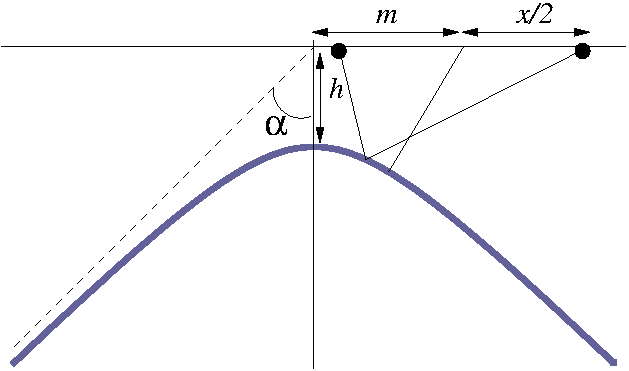
\includegraphics[width=0.31\columnwidth]{hyper/Fig/hyper}
    \label{fig:hyper}}    
  \subfloat[]{\includegraphics[width=0.31\columnwidth]{hyper/Fig/hyper-ct-0}
    \label{fig:hyper-ct}}
  \subfloat[]{\includegraphics[width=0.31\columnwidth]{hyper/Fig/hyper-fx-0}
    \label{fig:hyper-fx}}                
   \caption{\wen{Second synthetic example. (a) Clean data. (b) Denoised data using the proposed approach.  (c) Denoised data using the traditional seislet thresholding approach. (d) Noisy data. (e) Denoised data using the curvelet transform. (f) Denoised data using $f-x$ deconvolution.}}
   \label{fig:hyper-c,hyper-e,hyper-s,hyper,hyper-ct,hyper-fx}
\end{figure}

\begin{figure}[htb!]
  \centering
  \subfloat[]{\includegraphics[width=0.31\columnwidth]{hyper/Fig/hyper-e-n}
    \label{fig:hyper-e-n}}
  \subfloat[]{\includegraphics[width=0.31\columnwidth]{hyper/Fig/hyper-s-n-0}
    \label{fig:hyper-s-n-0}}\\
  \subfloat[]{\includegraphics[width=0.31\columnwidth]{hyper/Fig/hyper-ct-n-0}
    \label{fig:hyper-ct-n-0}}
  \subfloat[]{\includegraphics[width=0.31\columnwidth]{hyper/Fig/hyper-fx-n-0}
    \label{fig:hyper-fx-n}}    
   \caption{\wen{Removed noise sections for the second synthetic example. (a) Noise section using the proposed method. (b) Noise section using the conventional seislet thresholding method. (c) Noise section using the curvelet thresholding approach. (d) Noise section using $f-x$ deconvolution.}}
   \label{fig:hyper-e-n,hyper-s-n-0,hyper-ct-n-0,hyper-fx-n}
\end{figure}



\begin{figure}[htb!]
 \centering
 \subfloat[]{\includegraphics[width=0.31\columnwidth]{field/Fig/field}
   \label{fig:field}}
 \subfloat[]{\includegraphics[width=0.31\columnwidth]{field/Fig/field-emdseis}
   \label{fig:field-e}}
 \subfloat[]{\includegraphics[width=0.31\columnwidth]{field/Fig/field-recon}
   \label{fig:field-s}}\\
 \subfloat[]{\includegraphics[width=0.31\columnwidth]{field/Fig/field-ct}
   \label{fig:field-c}}
 \subfloat[]{\includegraphics[width=0.31\columnwidth]{field/Fig/field-fx}
   \label{fig:field-fx}}                
  \caption{\wen{(a) Field data. (b) Denoised data using the proposed approach. (c) Denoised data using the traditional seislet thresholding approach. (d) Denoised data using the curvelet transform. (e) Denoised data using $f-x$ deconvolution.}}
  \label{fig:field}
\end{figure}

\begin{figure}[htb!]
 \centering
 \subfloat[]{\includegraphics[width=0.48\columnwidth]{field/Fig/field-emdseis-dif}
   \label{fig:field-e-n}}
 \subfloat[]{\includegraphics[width=0.48\columnwidth]{field/Fig/field-seis-dif}
   \label{fig:field-s-n}}\\
 \subfloat[]{\includegraphics[width=0.48\columnwidth]{field/Fig/field-ct-dif}
   \label{fig:field-c-n}}
 \subfloat[]{\includegraphics[width=0.48\columnwidth]{field/Fig/field-fx-dif}
   \label{fig:field-fx-n}}    
  \caption{Removed noise sections for field data. (a) Noise section using the proposed method. (b) Noise section using the conventional seislet thresholding method. \wen{(c) Noise section using the curvelet thresholding approach. (d) Noise section using $f-x$ deconvolution.}}
  \label{fig:field-e-n,field-s-n,field-c-n,field-fx-n}
\end{figure}

\begin{figure}[htb!]
  \centering
  \subfloat[]{\includegraphics[width=0.48\columnwidth]{field/Fig/zoom2-emdseis}
    \label{fig:zoom2-emdseis}}
  \subfloat[]{\includegraphics[width=0.48\columnwidth]{field/Fig/zoom2-recon}
    \label{fig:zoom2-recon}}\\
  \subfloat[]{\includegraphics[width=0.48\columnwidth]{field/Fig/zoom1-emdseis}
    \label{fig:zoom1-emdseis}}
  \subfloat[]{\includegraphics[width=0.48\columnwidth]{field/Fig/zoom1-recon}
    \label{fig:zoom1-recon}}
   \caption{Zoomed denoised results for field data (corresponding to the frame boxes A \& B in Figure \ref{fig:field-sep1-recon,field-sep2-recon,field-emdseis,field-recon}). (a) \& (c) correspond to the proposed method. (b) \& (d) correspond to the conventional seislet thresholding method.}
   \label{fig:zoom2-emdseis,zoom2-recon,zoom1-emdseis,zoom1-recon}
\end{figure}


%\begin{figure}[htb!]
%  \centering
%  \subfloat[]{\includegraphics[width=0.31\columnwidth]{southsea/Fig/sc}
%    \label{fig:sc}}
%  \subfloat[]{\includegraphics[width=0.31\columnwidth]{southsea/Fig/sc-e}
%    \label{fig:sc-e}}
%  \subfloat[]{\includegraphics[width=0.31\columnwidth]{southsea/Fig/sc-s}
%    \label{fig:sc-s}}
%  \subfloat[]{\includegraphics[width=0.31\columnwidth]{southsea/Fig/sc-c}
%    \label{fig:sc-c}}
%  \subfloat[]{\includegraphics[width=0.31\columnwidth]{southsea/Fig/sc-fx}
%    \label{fig:sc-fx}}                
%   \caption{\wen{(a) sc data. (b) Denoised data using the proposed approach. (c) Denoised data using the traditional seislet thresholding approach. (d) Denoised data using the curvelet transform. (e) Denoised data using $f-x$ deconvolution.}}
%   \label{fig:sc}
%\end{figure}

%\begin{figure}[htb!]
%  \centering
%  \subfloat[]{\includegraphics[width=0.48\columnwidth]{southsea/Fig/sc-e-n}
%    \label{fig:sc-e-n}}
%  \subfloat[]{\includegraphics[width=0.48\columnwidth]{southsea/Fig/sc-s-n}
%    \label{fig:sc-s-n}}
%  \subfloat[]{\includegraphics[width=0.48\columnwidth]{southsea/Fig/sc-c-n}
%    \label{fig:sc-c-n}}
%  \subfloat[]{\includegraphics[width=0.48\columnwidth]{southsea/Fig/sc-fx-n}
%    \label{fig:sc-fx-n}}    
%   \caption{Removed noise sections for sc data. (a) Noise section using the proposed method. (b) Noise section using the conventional seislet thresholding method. \wen{(c) Noise section using the curvelet thresholding approach. (d) Noise section using $f-x$ deconvolution.}}
%   \label{fig:sc-emdseis-dif,sc-seis-dif,sc-curv-dif,sc-fx-dif}
%\end{figure}
}

\section{Conclusion}
I have proposed a novel \dlo{semi-automatic} dip-separated structural filtering approach that cascades a new empirical mode decomposition based adaptive dip filter and one structural filtering approach. The seislet thresholding is used as a simple example for structural filtering. The principle idea of the proposed approach is to adaptively separate complicated seismic profiles that contain dip conflicts into separated profiles that contain no dip conflicts. \dlo{The separation is achieved by two steps. The first step is to adaptively decompose the data into many dip components using the empirical mode decomposition based dip filter, and then manually combine the initial decomposed dip components into a smaller number of recombined dip components.}\wen{The dip separation is achieved by the empirical mode decomposition based dip filter.} \dlo{This first-decomposition and second-recombination dip separation strategy using the empirical mode decomposition based dip filter enjoys the benefits of convenience of adaptivity and efficiency for later seislet thresholding.} Because of the dip decomposition\dlo{ and recombination}, plane-wave destruction can obtain more precise slope estimation on each \dlo{recombined} dip component and can help to obtain better compression performance for the seislet transform than the traditional implementation. Synthetic and field data examples show that the proposed approach\dlo{ can not only help to preserve more useful energy and enhance weak signals, but also can increase the stability when using seislet-based thresholding}\wen{can help remove more random noise while preserving the energy of useful signals}.

\section{Acknowledgment}
I would like to thank Karl Schleicher, Shuwei Gan, Zhaoyu Jin, Sergey Fomel and Jianwei Ma for fruitful discussions. I also thank Jean Virieux and two anonymous reviewers for very constructive suggestions that improve the manuscript greatly. The paper was prepared in the Madagascar \cite[]{mada2013} open-source software platform and all the examples shown in the paper are reproducible.

\append{Review of \wen{EMD}\dlo{empirical mode decomposition} based dip filter}
The \dlo{EMD}\wen{empirical mode decomposition (EMD)} based dip filter is implemented in $f$-$x$ domain. As EMD \cite[]{emd,yangkang2015enhemd,shuwei20152} can empirically decompose a 1 D signal into different components that corresponds to different oscillating frequency, \dlo{we}\wen{one} can apply EMD to each frequency slice in $f$-$x$ domain and gather the same oscillating component\wen{s} for each frequency slice for separated $f$-$x$ domain profile. \dlo{We}\wen{One} then can get different separated seismic section\wen{s} by transforming the separated $f$-$x$ data back to $t$-$x$ domain. As the different oscillating components in each frequency slice of $f$-$x$ domain correspond to different dip components, the separating process acts as an adaptive dip filter.  

The formulation of the EMD based dip filter was given by \cite{yangkang2014}:
\wen{
\begin{equation}
\label{eq:emdbdf}
u(f,h)=\sum_{n=1}^{N}d_n(f,h),
\end{equation}
}
\dlo{where \dlo{$N$}\wen{$I$} is the number of decomposed \wen{intrinsic mode functions (IMFs)} \dlo{IMFs} in each frequency slice, $\Lambda(f,h)$ is the filtered data for frequency slice $f$ in the $f-x$ domain. \dlo{$u_i(f,h)(i=1,2,\cdots,N)$}\wen{$u_i(f,h)(i=1,2,\cdots,I)$} is the $i$th separated IMF such that $S(f,h)=\sum_{i=1}^{I}u_i(f,h)$, where $S(f,h)$ is the transformed $f-x$ domain seismic data. \dlo{$D_i(i=1,2,\cdots,M)$}\wen{$D_i(i=1,2,\cdots,N)$} is the $i$th dip band or component, and \dlo{$M$}\wen{$N$} is the number of dip bands or the number of dip components to be separated, and $\epsilon_i$ is the corresponding weighting coefficient. For a simple high-pass dip filter, we can choose \dlo{$M=2$, $\epsilon_1=1$, $\epsilon_2=0$ and $D_1=\{1,2\}$, $D_2=\{3,4,\cdots,N\}$.}\wen{$N=2$, $\epsilon_1=1$, $\epsilon_2=0$ and $D_1=\{1,2\}$, $D_2=\{3,4,\cdots,I\}$.} To form a dip filter that separates a seismic profile into five dip components, we can parameterize equation \ref{eq:emdbdf} as shown in Table \ref{tbl:filterpara1}. Note that, for every seismic data, we can use the same parameters as shown Table \ref{tbl:filterpara1} to obtained five dip components. To obtain a different number of dip components, we only need to specify the number of dip components \dlo{$M$}\wen{$N$} and parameterize equation \ref{eq:emdbdf} similarly.}
\wen{where $N$ is the number of dip components or the number of EMD decomposed components. $n$ denotes index, $f$ denotes frequency, and $h$ denotes spatial trace index. The decomposition is done in each frequency slice in the frequency-space domain via EMD. The details of EMD can be found in \cite{emd}. }

\wen{Equation \ref{eq:emdbdf} is formulated in the frequency domain in its original form. In the time-space domain, the EMD based dip filtering is simply
\begin{equation}
\label{eq:emdbdft}
\mathbf{u}=\sum_{n=1}^{N}\mathbf{d_n},
\end{equation}
where $\mathbf{u}$ is the vectorized seismic data, $\mathbf{d}_n$ is the $n$th dip component after using the EMD based dip filter. It is obvious that the EMD based dip filter is a linear transform and the summation of all the dip components is the original seismic image.
 }


%\tabl{filterpara1}{Parameters in designing 5 \dlo{EMDBDF}\wen{EMD based dip filter}s in order to separate seismic section into five dip components, as shown in Figures \ref{fig:dip1,dip2,dip3,dip4,dip5}\dlo{ and \ref{fig:field-dip1,field-dip2,field-dip3,field-dip4,field-dip5}}.}
% {
%    \begin{center}
%     \begin{tabular}{|c|c|c|c|c|}
%      \hline Filter index     & \dlo{$N$}\wen{$I$}  & \wen{$n$}\dlo{$m$}  & $\epsilon$   			        & $D$    		 \\ 
%      \hline first & 10   &2    & $\epsilon_1=1, \epsilon_2=0$ 		& $D_1=\{1\}, D_2=\{2,3,\cdots,10\}$ \\
%      \hline second  & 10   &3    & $\epsilon_1=0, \epsilon_2=1, \epsilon_3=0$& $D_1=\{1\}, D_2=\{2\}, D_3=\{3,4,\cdots,10\}$ \\
%      \hline third  & 10   &3    & $\epsilon_1=0, \epsilon_2=1, \epsilon_3=0$ 		& $D_1=\{1,2\}, D_2=\{3\}, D_3=\{4,5,\cdots,10\}$ \\
%      \hline fourth  & 10   &3    & $\epsilon_1=0, \epsilon_2=1, \epsilon_3=0$ 		& $D_1=\{1,2,3\}, D_2=\{4\}, D_3=\{5,6,\cdots,10\}$ \\
%      \hline fifth  & 10   &2    & $\epsilon_1=0, \epsilon_2=1$ 		& $D_1=\{1,2,3,4\}, D_2=\{5,6,\cdots,10\}$ \\
%      \hline
%    \end{tabular} 
%   \end{center}
%}
\onecolumn
\bibliographystyle{seg}
\bibliography{emdseis}

\newpage



